\documentclass[main.tex]{subfiles}
\begin{document}
%TODO: knowledge for functor subscripts?
%TODO: knowledge for symmetry groups.
%TODO: retract and section.
\chapter{Categories and Functors}\label{chap:catfunc}
\marginnote[-6\baselineskip]{
	\etocsettocstyle{}{}
	\etocsettocdepth{1}
	\localtableofcontents
}
As you will soon realize, many common mathematical objects can be viewed as "categories" or parts of a "category", and often in several ways. Hence, there can be many starting points to motivate category theory even after restricting ourselves to the background of an undergraduate student in mathematics (see Chapter \ref{chap:prelim}). I do not want to spend much time in the realm of informal explanations, so we will start from the notion of "directed graphs", quickly get to the definition of a "category" and begin an enumeration of examples which will carry on (implicitly) for the rest of the book. We will also define functors which are to categories what homomorphisms are to groups (or rings, etc.), and list a bunch of examples.
\section{Categories}

\begin{defn}[Directed graph]
	\AP A ""directed graph"" $G$ consists of a "collection" of ""nodes"" or ""objects"" denoted $\obj{G}$ and a "collection" of ""arrows"" or ""morphisms"" denoted $\mor{G}$ along with \AP two maps $\source,\target: \mor{G} \rightarrow \obj{G}$, so that each "arrow" $f \in \mor{G}$ has a ""source"" $\source(f)$ and a ""target"" $\target(f)$.\begin{marginfigure}We draw a "morphism" as an arrow, the "source" being its tail and "target" being its head:\begin{equation*}
		% https://q.uiver.app/?q=WzAsMixbMCwwLCJcXHNvdXJjZShmKSJdLFsxLDAsIlxcdGFyZ2V0KGYpIl0sWzAsMSwiZiJdXQ==
		\begin{tikzcd}
		{\source(f)} & {\target(f)}
		\arrow["f", from=1-1, to=1-2]
		\end{tikzcd}	
	\end{equation*}\end{marginfigure}
\end{defn}
\begin{defn}[Paths]
	\AP A ""path"" in a "directed graph" $G$ is a sequence of "arrows" $(f_1, \dots, f_k)$ that are ""composable"" in the sense that $\target(f_i) = \source(f_{i-1})$ for $i=2,\dots, k$ as drawn below in \eqref{diag:defpath}. The "collection" of "paths" of "length" $k$ in $G$ will be denoted $G_k$.\footnote{\AP The ""length"" of a "path" is the number of "arrows" in it. It is fitting that $\mor{G}$ denotes the "arrows" of $G$ and the "paths" of "length" $1$ in $G$ as they are the same thing.}
	\begin{equation}\label{diag:defpath}
		\begin{tikzcd}
			\bullet \arrow[r, "f_k"] & \bullet \arrow[r, "f_{k-1}"] & \bullet\cdots\bullet \arrow[r, "f_2"] & \bullet \arrow[r, "f_1"] & \bullet
		\end{tikzcd}
	\end{equation}
\end{defn}

Observe that when referring to a "path" as $(f_1,\dots, f_k)$ or drawing it as in \eqref{diag:defpath}, there is a mismatch in the ordering of the "arrows". The order as drawn --- also called the diagrammatic order --- agrees with the usual notation in graph theory (the branch of mathematics concerned with studying graphs), and it is arguably a more intuitive representation of the word ``"path"''. The other order will be motivated when we will define the "composition" of "arrows" in a "category". The main idea is that, conceptually, "arrows" coincide more closely with functions between mathematical objects, and if we see the "arrows" in \eqref{diag:defpath} as functions, their composition is most of the time denoted by $f_1 \circ \cdots \circ f_k$.
\begin{exmps}\label{exmps:digraphs}
	It is very simple to give an example of a "directed graph" by drawing a bunch of "nodes" and "arrows" between them as in \eqref{diag:orgraphexmp}, $\obj{G}$ is the "collection" of "nodes", $\mor{G}$ is the "collection" of "arrows" and $\source$ and $\target$ can be inferred from looking at the head and tail of each arrow. Let us give more examples to motivate the next definition.
	\begin{marginfigure}\begin{equation}\label{diag:orgraphexmp}
		% https://q.uiver.app/?q=WzAsNyxbMSwxLCJcXGJ1bGxldCJdLFsyLDIsIlxcYnVsbGV0Il0sWzMsMSwiXFxidWxsZXQiXSxbMywwLCJcXGJ1bGxldCJdLFsyLDEsIlxcYnVsbGV0Il0sWzAsMCwiXFxidWxsZXQiXSxbMSwwLCJcXGJ1bGxldCJdLFswLDFdLFsxLDJdLFsyLDNdLFszLDRdLFs0LDJdLFs1LDYsIiIsMCx7ImN1cnZlIjotMX1dLFs2LDUsIiIsMCx7ImN1cnZlIjotMX1dXQ==
		\begin{tikzcd}
			\bullet & \bullet && \bullet \\
			& \bullet & \bullet & \bullet \\
			&& \bullet
			\arrow[from=2-2, to=3-3]
			\arrow[from=3-3, to=2-4]
			\arrow[from=2-4, to=1-4]
			\arrow[from=1-4, to=2-3]
			\arrow[from=2-3, to=2-4]
			\arrow[curve={height=-6pt}, from=1-1, to=1-2]
			\arrow[curve={height=-6pt}, from=1-2, to=1-1]
		\end{tikzcd}
	\end{equation}\end{marginfigure}
	\begin{enumerate}
		\item For any set $X$, there is a trivial "directed graph" with $X$ as its "collection" of "nodes" and no "arrows". The "source" and "target" maps are the unique functions $\emptyset \rightarrow X$. You can represent it by drawing a "node" for each element of $X$.\footnote{This is a very uninteresting "directed graph".}
		
		There is a slightly more complex "directed graph" whose "nodes" are the elements of $X$. For each pair $(x,x') \in X \times X$, we can add an "arrow" with "source" $x$ and "target" $x'$. Drawing it is still fairly simple\footnote{Provided the set $X$ is finite}: you draw a "node" for each element of $X$ and an "arrow" from $x$ to $x'$ for each pair $(x,x')$.\footnote{Note that there are so-called ""loops"" which are "arrows" from a "node" to itself because $(x,x)$ is in $X \times X$.}
		\item Starting from a set $X$, we can define another "directed graph" by letting $X$ be its only "node" and the "collection" of "arrows" be the set of functions from $X$ to itself. The "source" and "target" maps are uniquely determined again, this time by their codomain that contains only the "node" $X$. This "graph@@DG" is already more interesting since the "collection" of "arrows" has a "monoid" structure. Indeed, the operation of composition of functions is associative, and the identity function is the identity for this operation.
		
		\item\label{exmp:digraphset} Taking inspiration from the previous examples, we define a "directed graph" $\mathbf{Set}$. It contains one "node" for every set, i.e., $\obj{\mathbf{Set}}$ is the "collection" of all sets, \footnote{Notice how we could not have defined this "graph@@DG" if we required $\obj{G}$ to be a set.} and one "arrow" with "source" $X$ and "target" $Y$ for every function $f: X \rightarrow Y$. 
		
		Similarly to the last example, we recognize that the "collection" of "arrows" has a novel kind of structure induced by composition of functions and identity functions. It is not a "monoid" because you can only compose functions when one's "source" is the "target" of the other. In other words, composition of functions is not a binary operation $\circ : \mor{\mathbf{Set}} \times \mor{\mathbf{Set}} \rightarrow \mor{\mathbf{Set}}$, it is of type $\mortwo{\mathbf{Set}} \rightarrow \mor{\mathbf{Set}}$. Nonetheless, we still have associativity and identities which are at the core of the definition of a "monoid". Since the theory of "monoids" is extremely rich and ubiquitous in mathematics, it is daring to study this seemingly more complex variant. We first need to make this structure abstract in the definition of a "category".
	\end{enumerate}
\end{exmps}


\begin{defn}[Category]\label{defn:cat}
	\AP A "directed graph" $\mathbf{C}$ along with a ""composition"" map $\circ: \mortwo{\mathbf{C}} \rightarrow \mor{\mathbf{C}}$ is a ""category"" if it satisfies the following properties:
	\begin{enumerate}
		\item For any $(f, g) \in \mortwo{\mathbf{C}}$, $\source(f \circ g) = \source(g)$ and $\target(f \circ g) = \target(f)$. This is more naturally understood visually in \eqref{diag:stcomp}.\begin{marginfigure}\begin{equation}\label{diag:stcomp}
			\begin{tikzcd}
				\bullet \arrow[r, "g"'] \arrow[rr, "f \circ g", bend left] & \bullet \arrow[r, "f"'] & \bullet
			\end{tikzcd}
		\end{equation}\end{marginfigure}
		\item For any $(f,g,h) \in \mathbf{C}_3$, $f\circ(g\circ h) = (f\circ g)\circ h$, namely, "composition" is "associative". Again, the graphic representation in \eqref{diag:assoccomp} may be more revealing. \begin{marginfigure}\begin{equation}\label{diag:assoccomp}
			% https://q.uiver.app/?q=WzAsNCxbMCwwLCJcXGJ1bGxldCJdLFsxLDAsIlxcYnVsbGV0Il0sWzIsMCwiXFxidWxsZXQiXSxbMywwLCJcXGJ1bGxldCJdLFswLDEsImgiLDFdLFsxLDIsImciLDFdLFsyLDMsImYiLDFdLFsxLDMsImYgXFxjaXJjIGciLDEseyJjdXJ2ZSI6LTJ9XSxbMCwzLCIoZiBcXGNpcmMgZykgXFxjaXJjIGgiLDEseyJjdXJ2ZSI6LTV9XSxbMCwyLCJnXFxjaXJjIGgiLDEseyJjdXJ2ZSI6Mn1dLFswLDMsImYgXFxjaXJjIChnIFxcY2lyYyBoKSIsMSx7ImN1cnZlIjo1fV1d
			\begin{tikzcd}
				\bullet & \bullet & \bullet & \bullet
				\arrow["h"{description}, from=1-1, to=1-2]
				\arrow["g"{description}, from=1-2, to=1-3]
				\arrow["f"{description}, from=1-3, to=1-4]
				\arrow["{f \circ g}"{description}, curve={height=-12pt}, from=1-2, to=1-4]
				\arrow["{(f \circ g) \circ h}"{description}, curve={height=-30pt}, from=1-1, to=1-4]
				\arrow["{g\circ h}"{description}, curve={height=12pt}, from=1-1, to=1-3]
				\arrow["{f \circ (g \circ h)}"{description}, curve={height=30pt}, from=1-1, to=1-4]
			\end{tikzcd}
		\end{equation}\end{marginfigure}
		\item For any "object" $A \in \obj{\mathbf{C}}$, there exists an ""identity"" morphism $\idu_{\mathbf{C}}(A) \in \mor{\mathbf{C}}$ with $A$ as its "source" and "target" that satisfies $\idu_{\mathbf{C}}(A) \circ f = f$ and $g \circ \idu_{\mathbf{C}}(A) = g$, for any $f,g \in \mor{\mathbf{C}}$ where $\target(f) = A$ and $\source(g) = A$.
	\end{enumerate}
\end{defn}
\marginnote{\AP If the third property of Definition \ref{defn:cat} is not satisfied, $\mathbf{C}$ is referred to as a ""semicategory"". In rare occasions, authors choose to explicit when a category \emph{does} satisfy this property, qualifying it as unital.}
\begin{rem}[Notation]
	In general, we will refer to "categories" with bold uppercase letters typeset with \verb!\mathbf! ($\mathbf{C}$, $\mathbf{D}$, $\mathbf{E}$, etc.), their "objects" with uppercase letters ($A$, $B$, $X$, $Y$, $Z$, etc.) and their "morphisms" with lowercase letters ($f$, $g$, $h$, etc.). When the "category" is clear from the context, we denote the "identity" "morphisms" $\id_A$ instead of $\idu_{\mathbf{C}}(A)$. \AP We say that two "morphisms" are ""parallel"" if they have the same "source" and "target". \AP Given "morphisms" $f$ and $g$ in a "category" $\mathbf{C}$, we say that $f$ ""factors through"" $g$ if there exists $h\in \mor{\mathbf{C}}$ such that $f = g \circ h$ or $f = h \circ g$.
\end{rem}

Observe that since $\circ$ is "associative", it induces a unique \kl[comppaths]{composition} map on "paths" of any finite "lengths", which we abusively denote $\circ: \mathbf{C}_k \rightarrow \mor{\mathbf{C}}$.\footnote{Another abuse we make is to define $\circ: \obj{\mathbf{C}} \rightarrow \mor{\mathbf{C}}$ by $X \mapsto \id_X$. That is, we identify "objects" of $\mathbf{C}$ with empty "paths" (of "length" $0$) starting and ending at that "object", and we consider the "composition@comppaths" of an empty "path" to be the "identity".} This lets us write $f_1 \circ f_2 \circ \cdots \circ f_k$ with no parentheses. \AP Occasionally, we will refer to the image of the path under this map as the \intro[comppaths]{composition of the path} or the \reintro[comppaths]{morphism that a path composes to}.
\begin{exmps}[Boring examples]\label{exmp:simplecats}
	\begin{marginfigure}[5\baselineskip]\begin{equation}\label{diag:cat1}\begin{tikzcd}\bullet \arrow[loop, distance=2em, in=55, out=125]\end{tikzcd}\end{equation}\end{marginfigure} 
	It can be really easy to construct a "category" by drawing its underlying "directed graph" and inferring the definition of the "composition" from it. Starting from the very simple "graph@@DG" depicted in \eqref{diag:cat1}, we can infer the definition of a "category" with a single "object" and its "identity morphism". \AP This "category" is denoted $\intro*\termcat$, the "composition" is trivial since $\id_{\bullet} \circ \id_{\bullet} = \id_{\bullet}$.

	\begin{marginfigure}[1\baselineskip]\begin{equation}\label{diag:cat1p1}\begin{tikzcd}\bullet_1 \arrow[loop, distance=2em, in=55, out=125]&\bullet_2 \arrow[loop, distance=2em, in=55, out=125]\end{tikzcd}\end{equation}\end{marginfigure}
	Similarly, we construct from the "graph@@DG" in \eqref{diag:cat1p1} a "category" with two "objects", their "identity morphisms" and nothing else. The "composition" is again trivial. This category will be denoted $\termcat \coproduct \termcat$.\footnote{This notation is cleared up in Definition \ref{defn:coproduct}.}
	More generally, for any "collection" $\obj{\mathbf{C}}$, there is a "category" $\mathbf{C}$ whose "collection" of "objects" is $\obj{\mathbf{C}}$ and whose "collection" of "morphisms" is $\mor{\mathbf{C}} := \{\id_X \mid X \in \obj{\mathbf{C}}\}$. The "composition map" is completely determined by the third property in Definition \ref{defn:cat}.\footnote{i.e., for any $X \in \obj{\mathbf{C}}$, $\id_X \circ \id_X = \id_X$.} \AP A "category" without non-"identity morphisms" is called a ""discrete category"".
	
	The "graph@@DG" in \eqref{diag:cat2} corresponds to the "category" with "objects" $\{A, B\}$ and "morphisms" $\{\id_A, \id_B, f\}$.
	\begin{equation}\label{diag:cat2}
		\begin{tikzcd}
			A \arrow[r, "f"] \arrow["\id_A", loop, distance=2em, in=145, out=215] & B \arrow["\id_B"', loop, distance=2em, in=35, out=325]
		\end{tikzcd}
	\end{equation}
	The "composition map" is then completely determined by the properties of "identity morphisms".\footnote{i.e., $f \circ \id_A = f$, $\id_B \circ f = f$, $\id_A \circ \id_A = \id_A$ and $\id_B \circ \id_B = \id_B$} \AP This "category" is called the "interval category" or the \textbf{"walking arrow"}, and it is denoted $\intro*\cattwo$. Note however that $\termcat \coproduct \termcat \neq \cattwo$.
	
	Starting now, we will omit the "identity morphisms" from the diagrams (as is usual in the literature) for clarity reasons: they would hinder readability without adding information.
	
	It is not always as straightforward to construct a "category" from a "directed graph". For instance, if two distinct "arrows" have the same "source" and "target", they must be explicitly drawn and the ambiguity in the "composition" must be dealt with. The "graph@@DG" in \eqref{diag:ambsquare} is problematic in this way: it has two distinct "paths" of "length" two starting at the top-left corner and ending at the bottom-right corner. Since the \kl[comppaths]{composition} of these "paths" can be equal to any of the two distinct "morphisms" between these corners, there is no "category" obviously corresponding to this "graph@@DG".\begin{marginfigure}[-5\baselineskip]\begin{equation}\label{diag:ambsquare}\begin{tikzcd}
		\bullet \arrow[r] \arrow[d] \arrow[rd, shift left] \arrow[rd, shift right] & \bullet \arrow[d] \\
		\bullet \arrow[r]                                                          & \bullet          
		\end{tikzcd}\end{equation}\end{marginfigure}
\end{exmps}
Since "categories" can be quite huge, it is rare that we draw all of a "category" at once. We will often draw diagrams with (labelled) "nodes" and "arrows" to represent the "objects" and "morphisms" within a "category" that we are focusing on. We also omit from our diagrams "morphisms" that can be inferred from the categorical structure. For instance, if we draw two "composable" "morphisms" as in \eqref{diag:twocompose}, we do not draw the "identity morphisms" nor the "composition" $g \circ f$.
\begin{marginfigure}[-5\baselineskip]
	% https://q.uiver.app/?q=WzAsMyxbMCwwLCJBIl0sWzEsMCwiQiJdLFsyLDAsIkMiXSxbMCwxLCJmIl0sWzEsMiwiZyJdXQ==
	\begin{equation}\label{diag:twocompose}
		\begin{tikzcd}
			A & B & C
			\arrow["f", from=1-1, to=1-2]
			\arrow["g", from=1-2, to=1-3]
		\end{tikzcd}
	\end{equation}
\end{marginfigure}
In many cases, not drawing all "morphisms" can lead to ambiguities like for \eqref{diag:ambsquare}. We have to be careful to avoid these, but sometimes we can resolve the problem by stating that the diagram is \textbf{"commutative"}.
\begin{defn}[Commutativity]\label{defn:commutative}
	\AP Given a diagram representing "objects" and "morphisms" in a "category", we say that it is ""commutative"" if the "composition@comppaths" of any "path" of "length" greater than one is equal to the "composition@comppaths" of any other "path" with the same "source" and "target". The "morphism" resulting from the "composition@comppaths" may or may not be depicted.
\end{defn}
\begin{exmps}
	Arguably the most frequently used "commutative diagram" is the "commutative" square drawn in \eqref{diag:commusquare}.
	\begin{equation}\label{diag:commusquare}\begin{tikzcd}
		\bullet \arrow[r] \arrow[d] & \bullet \arrow[d] \\
		\bullet \arrow[r]           & \bullet          
	\end{tikzcd}\end{equation}
	We say the square "commutes" when the bottom and top "paths" \kl[comppaths]{compose to} the same (omitted in the diagram) "morphism". The "commutative" square can also be seen as a "category" by inferring the missing "morphism" and the "composition" from "commutativity". We can denote it $\cattwo \cattimes \cattwo$.\footnote{This notation is explained in Definition \ref{defn:prodcat}.}
	\begin{marginfigure}\begin{equation}\label{diag:twocommsquare}
		% https://q.uiver.app/?q=WzAsNixbMCwwLCJcXGJ1bGxldCJdLFswLDEsIlxcYnVsbGV0Il0sWzEsMSwiXFxidWxsZXQiXSxbMSwwLCJcXGJ1bGxldCJdLFsyLDAsIlxcYnVsbGV0Il0sWzIsMSwiXFxidWxsZXQiXSxbMCwxLCJoIiwyXSxbMSwyLCJmJyIsMl0sWzAsMywiZiJdLFszLDQsImciXSxbMiw1LCJnJyIsMl0sWzQsNSwiaCcnIl0sWzMsMiwiaCciLDJdXQ==
		\begin{tikzcd}
			\bullet & \bullet & \bullet \\
			\bullet & \bullet & \bullet
			\arrow["h"', from=1-1, to=2-1]
			\arrow["{f'}"', from=2-1, to=2-2]
			\arrow["f", from=1-1, to=1-2]
			\arrow["g", from=1-2, to=1-3]
			\arrow["{g'}"', from=2-2, to=2-3]
			\arrow["{h''}", from=1-3, to=2-3]
			\arrow["{h'}"', from=1-2, to=2-2]
		\end{tikzcd}
	\end{equation}\end{marginfigure}
	Assuming that \eqref{diag:twocommsquare} "commutes", we can infer that $f' \circ h = h' \circ f$, $g' \circ h' = h'' \circ g$, and $g' \circ f' \circ h = h'' \circ g \circ f$. Observe that the last equation can be derived from the first two which are equivalent to the "commutativity" of the two squares in \eqref{diag:twocommsquare}. More generally, combining "commutative diagrams" in this way yields "commutative diagrams", and this is the core of a powerful proof method called "diagram paving" that we introduce at the end of this chapter.
	\begin{marginfigure}\begin{equation}\label{diag:twoparcomm}
		% https://q.uiver.app/?q=WzAsMixbMCwwLCJBIl0sWzEsMCwiQiJdLFswLDEsImYiLDAseyJvZmZzZXQiOi0xfV0sWzEsMCwiZyIsMCx7Im9mZnNldCI6LTF9XV0=
		\begin{tikzcd}
			A & B
			\arrow["f", shift left=1, from=1-1, to=1-2]
			\arrow["g", shift left=1, from=1-2, to=1-1]
		\end{tikzcd}
	\end{equation}\end{marginfigure}
	Stating that \eqref{diag:twoparcomm} "commutes" is equivalent to stating that $f \circ g \circ f = f$ and $g \circ f \circ g = g$. We can also infer that $f \circ g \circ f \circ g = f \circ g$ and $g \circ f \circ g \circ f = g \circ f$, but this follows from the first two equality.
	
	It would be odd to require that \eqref{diag:ambsquare} "commutes". It would imply that the two "parallel" "morphisms" are equal because they are both equal to the "composition@comppaths" of the bottom and top "paths". We will never draw "parallel" "morphisms" when they are supposed to be equal.
	
	To assert that two "morphisms" $f,g : A \rightarrow B$ are equal using a diagram, we can say that either of the following is "commutative", with a preference for the third one.\footnote{The equal sign in the third one can be read as $\id_A$ going in either direction.}
	\begin{equation}\label{diag:commuteparallel}
		% https://q.uiver.app/?q=WzAsOSxbMCwwLCJBIl0sWzEsMSwiQiJdLFswLDEsIkEiXSxbMiwwLCJBIl0sWzIsMSwiQSJdLFszLDEsIkIiXSxbNCwwLCJBIl0sWzQsMSwiQSJdLFs1LDEsIkIiXSxbMCwxLCJmIl0sWzIsMSwiZyIsMl0sWzAsMiwiXFxpZF9BIiwyXSxbNCw1LCJnIiwyXSxbMyw1LCJmIl0sWzYsNywiIiwyLHsibGV2ZWwiOjIsInN0eWxlIjp7ImhlYWQiOnsibmFtZSI6Im5vbmUifX19XSxbNyw4LCJnIiwyXSxbNiw4LCJmIl0sWzQsMywiXFxpZF9BIl1d
	\begin{tikzcd}
		A && A && A \\
		A & B & A & B & A & B
		\arrow["f", from=1-1, to=2-2]
		\arrow["g"', from=2-1, to=2-2]
		\arrow["{\id_A}"', from=1-1, to=2-1]
		\arrow["g"', from=2-3, to=2-4]
		\arrow["f", from=1-3, to=2-4]
		\arrow[Rightarrow, no head, from=1-5, to=2-5]
		\arrow["g"', from=2-5, to=2-6]
		\arrow["f", from=1-5, to=2-6]
		\arrow["{\id_A}", from=2-3, to=1-3]
	\end{tikzcd}
	\end{equation}	
\end{exmps}
\begin{rem}[Convention]
	Reasoning with "commutative diagrams" is an acquired skill we will practice quite a lot in the following chapters. Yet there is no standard definition that everyone systematically uses.\footnote{This does not really lead to many misunderstandings anyway because what is meant by a diagram is usually made clear by the context.} For this reason, I decided to pick my favorite definition of "commutativity" which is uncommon.\footnote{I have not seen the constraint on the "length" anywhere else.} In most cases, a diagram is called "commutative" when any two "paths" "compose@comppaths" to the same "morphism", but in practice, there are two exceptions handled by Definition \ref{defn:commutative}: %TODO: Begin category theory by Peter Smith has the same condition.
	\begin{enumerate}
		\item Two "parallel" "morphisms" are not always equal in a "commutative diagram". In fact, when "parallel" "morphisms" are drawn, it is usually to emphasize that they are distinct.
		\item Unless otherwise stated, an "endomorphism"\footnote{\AP An ""endomorphism"" is a "morphism" whose "source" and "target" coincide.} drawn in a "commutative diagram" is not equal to the "identity morphism" (the "composition@comppaths" of the empty "path").
	\end{enumerate}
\end{rem}
\begin{warn}
	Diagrams are not "commutative" by default. We will always specify when a diagram "commutes". As our usage of "commutative diagrams" ramps up in the following chapters, you have to try to remember that. 
\end{warn}

Before moving on to more interesting "categories", we introduce the $\Hom$ notation.
\begin{defn}[$\Hom$]
	\AP Let $\mathbf{C}$ be a "category" and $A,B \in \obj{\mathbf{C}}$ be "objects", the "collection" of all "morphisms" going from $A$ to $B$ is 
	\[\intro*\Hom_{\mathbf{C}}(A,B) := \{f \in \mor{\mathbf{C}} \mid \source(f) = A \text{ and } \target(f) = B\}.\]
	This leads to an alternative way of defining the "morphisms" of $\mathbf{C}$, namely, one can describe $\Hom_{\mathbf{C}}(A,B)$ for all $A, B \in \obj{\mathbf{C}}$ instead of describing $\mor{\mathbf{C}}$ all at once. Defining the "morphisms" this way also takes care of the "source" and "target" functions implicitly.
\end{defn}
\begin{rem}[Notation]
    Some authors choose to denote the "collection" of "morphisms" between $A$ and $B$ with $\mathbf{C}(A,B)$. I prefer to use the latter notation when working with "$2$--categories@2cat"\footnote{see Definition \ref{defn:2cat}.} to highlight the fact that $\mathbf{C}(A,B)$ has more structure. Other authors use $\mathrm{hom}$ with a lowercase ``h'', my choice here is arbitrary.
\end{rem}
\begin{defn}[Smallness]
	\AP A "category" $\mathbf{C}$ is called ""small"" if the "collections" of "objects" and "morphisms" are sets. \AP If for all "objects" $A,B \in \obj{\mathbf{C}}$, $\Hom_{\mathbf{C}}(A,B)$ is a set, $\mathbf{C}$ is said to be ""locally small"" and $\Hom_{\mathbf{C}}(A,B)$ is called a ""hom-set"". \AP A "category" that is not "small" can be referred to as ""large"".%TODO: footnote about foundation.
\end{defn}
The following three examples will follow us throughout the book.
\begin{exmp}[$\catSet$]
	\AP The "category" $\intro*\catSet$ has the "collection" of sets as its "objects" and for any sets $X$ and $Y$, $\Hom_{\catSet}(X,Y)$ is the set of all the functions from $X$ to $Y$.\footnote{We already saw this "directed graph" in Example \ref{exmps:digraphs}.\ref{exmp:digraphset}.} The "composition map" is given by composition of functions (which is "associative") and the identity maps serve as the "identity morphisms". This "category" is "locally small" but not "small".\footnote{By our argument at the start of Chapter \ref{chap:prelim}: the "collection" of all sets cannot be a set.}
	
	We will carry out many examples using $\catSet$ because it is elaborate enough to be interesting, yet it is easy to understand because we are (assumed to be) very familiar with sets and functions.
\end{exmp}
\begin{exmp}
	Let $(X, \leq)$ be a "partially ordered set", it can be viewed as a "category" with elements of $X$ as its "objects". For any $x,y \in X$, the "hom-set" $\Hom_X(x,y)$ contains a single "morphism" if $x \leq y$ and is empty otherwise. The "identity morphisms" arise from the "reflexivity" of $\leq$. Since every "hom-set" contains at most one element and $\leq$ is "transitive", the "composition map" is completely determined. Detailing this out, if $f:x \rightarrow y$ and $g: y \rightarrow z$ are "morphisms", then we know that $x \leq y$ and $y\leq z$. Thus, "transitivity" implies that $x\leq z$ and there is a unique "morphism" $x \rightarrow z$, so it must be $g \circ f$.\footnote{Note that "antisymmetry" was not used in this argument, so one can more generally construct a "category" starting from a "preorder". \AP Such "categories" are called ""thin"" because each "hom-set" contains at most one "morphism". It is straightforward to show the "identities" and "composition" ensure that any "thin" "category" $\mathbf{C}$ is constructed from the "preorder" $(\obj{\mathbf{C}}, \leq)$ with \[X \leq Y \Leftrightarrow \Hom_{\mathbf{C}}(X,Y) \neq \emptyset.\]}
	
	\AP If a "category" corresponds to this construction for some "poset", it is called ""posetal"". In \eqref{diag:natposet}, we depict the "posetal" "category" associated to $(\N, \leq)$. The "arrows" between numbers $n$ and $n+k$ are omitted for $k>1$ as they can be inferred by the "composition" $n \leq n+1 \leq n+2 \leq \cdots \leq n+k$.
	\begin{equation}\label{diag:natposet}
		\begin{tikzcd}
			\stackrel{0}{\bullet} \arrow[r] & \stackrel{1}{\bullet} \arrow[r] & \stackrel{2}{\bullet} \arrow[r] & \cdots
		\end{tikzcd}
	\end{equation}
	
	As a particular case of "posetal" "categories", let $(X, \tau)$ be a "topological space" and note that the inclusion relation on "open sets" is a "partial order" on $\tau$. Thus, $X$ has a corresponding "posetal" "category". More explicitly, the "objects" are "open sets" and for any $U, V \in \tau$, the "hom-set" $\Hom_X(U,V)$ contains the inclusion map $i_{UV}$ if $U\subseteq V$ and is empty otherwise. \AP This category will be denoted $\intro*\catOpens(X,\tau)$ or $\catOpens(X)$.

	We will carry out many examples using "posetal" "categories" because it avoids difficulties arising from having different "parallel" "morphisms".\footnote{For the same reason, "thin" "categories" are also simple cases to carry out examples with.} In particular, every diagram drawn with "objects" and "morphisms" from a "posetal" "category" is "commutative" because the "composition@comppaths" of any "path" is equal to the unique "morphism" between the "source" and "target" of that "path". This also means some important aspects of a concept can be trivial when instantiating it for a "posetal" "category".
\end{exmp}
\begin{exmp}[Single object categories]\label{exmp:monoid}
	\AP If a "category" $\mathbf{C}$ has a single "object" $\intro*\deloopobject$, then all "morphisms" go from $\deloopobject$ to $\deloopobject$. In particular, $\mor{\mathbf{C}} = \Hom_{\mathbf{C}}(\deloopobject, \deloopobject)$ and $\mortwo{\mathbf{C}} = \mor{\mathbf{C}} \times \mor{\mathbf{C}}$. Then, the "associativity" of $\circ$ and existence of $\id_{\deloopobject}$ make $(\mor{\mathbf{C}}, \circ)$ into a "monoid".
	
	Conversely, a "monoid" $(M, \cdot)$ can be represented by a single "object" "category" $M$, where $\Hom_M(\deloopobject, \deloopobject) = M$ and the "composition map" is the "monoid" operation.
	
	Since many algebraic structures have an "associative" operation  with an identity element, this yields a fairly general construction. \AP The single "object" "category" associated to a "monoid" or "group" $G$ will be denoted by $\deloop{G}$ and referred to as the \intro{delooping} of $G$.
		\begin{marginfigure}
		\begin{center}
			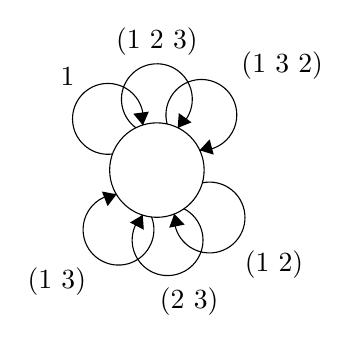
\begin{tikzpicture}[scale=0.2]
			\tikzstyle{every node}+=[inner sep=0pt]
			\draw [black] (37.4,-25.7) circle (3);
			\draw (37.4,-25.7) node {$\deloopobject$};
			\draw [black] (34.593,-24.676) arc (277.6886:-10.3114:2.25);
			\draw (31.72,-20.34) node [above] {$1$};
			\fill [black] (36.51,-22.85) -- (36.89,-21.99) -- (35.9,-22.12);
			\draw [black] (40.276,-26.512) arc (101.97044:-186.02956:2.25);
			\draw (42.95,-31.68) node [right] {$(1\ 2)$};
			\fill [black] (38.51,-28.48) -- (38.18,-29.36) -- (39.16,-29.16);
			\draw [black] (39.111,-28.15) arc (62.6723:-225.3277:2.25);
			\draw (39.45,-33.13) node [below] {$(2\ 3)$};
			\fill [black] (36.5,-28.55) -- (35.69,-29.03) -- (36.57,-29.49);
			\draw [black] (37.059,-28.669) arc (21.17668:-266.82332:2.25);
			\draw (31.05,-31.87) node [below] {$(1\ 3)$};
			\fill [black] (34.84,-27.24) -- (33.91,-27.06) -- (34.27,-27.99);
			\draw [black] (36.077,-23.02) arc (234:-54:2.25);
			\draw (37.4,-18.45) node [above] {$(1\ 2\ 3)$};
			\fill [black] (38.72,-23.02) -- (39.6,-22.67) -- (38.79,-22.08);
			\draw [black] (38.053,-22.784) arc (195.11223:-92.88777:2.25);
			\draw (45.36,-19.95) node [above] {$(1\ 3\ 2)$};
			\fill [black] (40.11,-24.44) -- (41.01,-24.72) -- (40.75,-23.75);
			\end{tikzpicture}
		\end{center}
		\caption{The "delooping" of the symmetric group $S_3$, a.k.a. $\deloop{S_3}$.}
	\end{marginfigure}
	
	The natural numbers can also be endowed with the "monoid" structure of addition, hence a particular instance of a single object "category" is the "delooping" of $(\N, +)$. Notice that this "category" is very different from the "posetal" "category" $(\N, \leq)$. In the former, $\N$ is in correspondence with the "morphisms" while in the latter, it is in correspondence with the "objects".
	
	We will carry out many examples using "deloopings" of "monoids" or "groups" because it avoids difficulties arising from having two different "objects".
\end{exmp}
Several simple examples of "large" "categories" arise as "subcategories" of $\catSet$.
\begin{defn}[Subcategory]
	\AP Let $\mathbf{C}$ be a "category", a "category" $\mathbf{C}'$ is a ""subcategory"" of $\mathbf{C}$ if, the following properties are satisfied.
	\begin{enumerate}
		\item The "objects" and "morphisms" of $\mathbf{C}'$ are "objects" and "morphisms" of $\mathbf{C}$ (i.e., $\obj{\mathbf{C}'} \subseteq \obj{\mathbf{C}}$ and $\mor{\mathbf{C}'} \subseteq \mor{\mathbf{C}}$).
		\item The "source" and "target" maps of $\mathbf{C}'$ are the restrictions of the "source" and "target" maps of $\mathbf{C}$ on $\mor{\mathbf{C}'}$ and for every morphism $f \in \mor{\mathbf{C}'}$, $\source(f), \target(f) \in \obj{\mathbf{C}'}$.
		\item The "composition map" of $\mathbf{C}'$ is the restriction of the "composition map" of $\mathbf{C}$ on $\mortwo{\mathbf{C}'}$ and for any $(f,g) \in \mortwo{\mathbf{C}'}$, $f\circ_{\mathbf{C}'} g = f \circ_{\mathbf{C}} g \in \mor{\mathbf{C}'}$.
		\item The "identity morphisms" of "objects" in $\obj{\mathbf{C}'}$ are the "identity morphisms" of "objects" in $\obj{\mathbf{C}}$, i.e., $\idu_{\mathbf{C}}(A) = \idu_{\mathbf{C}'}(A)$ when $A \in \obj{\mathbf{C}'}$.
	\end{enumerate}
	Intuitively, one can see $\mathbf{C}'$ as being obtained from $\mathbf{C}$ by removing some "objects" and "morphisms", but making sure that no "morphism" is left with no "source" or no "target" and that no "path" is left without its \kl[comppaths]{composition}.
\end{defn}
\begin{exer}{soln:catfunc:countersubcat}[\NOW]\label{exer:catfunc:countersubcat}
	Find an example of a "category" $\mathbf{C}$ and a "category" $\mathbf{C}'$ that satisfy the first three conditions but not the fourth.
\end{exer}
\begin{defn}[Full and wide]
	\AP A "subcategory" $\mathbf{C}'$ of $\mathbf{C}$ is called ""full@@CAT"" if for any "objects" $A,B \in \obj{\mathbf{C}'}$, $\Hom_{\mathbf{C}'}(A,B) = \Hom_{\mathbf{C}}(A,B)$. \AP It is called ""wide"" if $\obj{\mathbf{C}'} = \obj{\mathbf{C}}$.\footnote{In words, a "subcategory" is "full@@CAT" if the "morphisms" that were removed had their "source" or "target" removed as well, and it is "wide" if no "objects" were removed.}
\end{defn}
\begin{exmps}[Subcategories of $\catSet$]\label{exmp:subcatSet}
	We can selectively remove some "objects" and "morphisms" in $\catSet$ to obtain the following "categories".
	\begin{enumerate}
		\item Since the composition of injective functions is again injective, the restriction of morphisms in $\catSet$ to injective functions yields a "wide" "subcategory" of $\catSet$, denoted by $\intro*\catSetInj$. Unsurprisingly, $\intro*\catSetSurj$ can be constructed similarly.
		\item Removing all infinite sets from $\catSet$ yields the "full@@CAT" "subcategory" of finite sets denoted $\catFinSet$.\footnote{This "category" is not "small" because there is \href{https://math.stackexchange.com/questions/896270/collection-of-all-finite-sets}{no set of all finite sets}.}
		\item Further removing sets from $\catFinSet$ and keeping only $\emptyset$, $\{1\}$, $\{1,2\}$, $\{1,2,3\}$, etc., we obtain the "category" $\intro*\catFinOrd$ which is a "small" "full@@CAT" "subcategory" of $\catSet$.\footnote{The name $\catFinOrd$ is an abbreviation of finite \href{https://en.wikipedia.org/wiki/Ordinal_number}{ordinals}, because we can also define $\catFinOrd$ as the "category" of finite ordinals and functions between them.}
		\item Since the composition of "monotone" maps is "monotone" and the identity function is "monotone", we can view each set $\{1,\dots, n\}$ as ordered with $\leq$ and remove all "morphisms" that are not "monotone" from $\catFinOrd$. The resulting "category" is called the ""simplex category"" and denoted by $\catSimplex$.
	\end{enumerate}
\end{exmps}
\begin{exmps}[Concrete categories]\label{exmp:concreteCat}
	This second list of examples contains so-called "concrete categories". Informally, they are "categories" of sets with extra structure, where "morphisms" are functions that preserve that extra structure.\footnote{Formally, see Definition \ref{defn:concrete}.}
	\begin{enumerate}
		\itemAP The "category" $\catPtd$ is the "category" of ""pointed"" sets. Its "objects" are sets with a distinguished element, and its "morphisms" are functions that map distinguished elements to distinguished elements. The distinguished element of a pointed set is the extra structure on top of the set, and "morphisms" between pointed set must preserve that structure. In more details, $\obj{(\catPtd)}$ is the "collection" of pairs $(X,x)$ where $X$ is a set and $x \in X$, and for any two "pointed" sets $(X,x)$ and $(Y,y)$, 
		\[\Hom_{\catPtd}((X,x), (Y,y)) = \left\{ f: X \rightarrow Y \mid f(x) = y \right\}.\]
		The "identity morphisms" and "composition" are defined as in $\catSet$, so the axioms of a "category" clearly hold after checking that if $f:(X,x) \rightarrow (Y,y)$ satisfies $f(x) =y$ and $g: (Y,y) \rightarrow (Z,z)$ satisfies $g(y) = z$, then $(g\circ f)(x) = z$.
		\itemAP The "category" $\intro*\catMon$ is the "category" of "monoids" and their "homomorphisms@@MON", let us be more explicit.\footnote{These technicalities are essentially the same for the "categories" in the remainder of Example \ref{exmp:concreteCat}.} The "objects" are "monoids", so $\obj{\catMon}$ is the "collection" of all "monoids", and the "morphisms" are "monoid homomorphisms", so for any $M, N \in \obj{\catMon}$, $\Hom_{\catMon}(M,N)$ is the set of "homomorphisms@@MON" from $M$ to $N$. The "composition" in $\catMon$ is given by the composition of "homomorphisms@@MON", we know it is well-defined because the composition of two "homomorphisms@@MON" is a "homomorphism@@MON". Also, the "composition" is "associative" and the identity functions are "homomorphisms@@MON", so we can define $\idu_{\catMon}(M) = \mathrm{id}_M$.
		\itemAP Similarly, the "category" of "groups" (resp.\ "rings" or "fields") where the "morphisms" are "group" (resp.\ "ring" or "field") "homomorphisms@@GRP" is $\intro*\catGrp$ (resp.\ $\intro*\catRing$ or $\intro*\catField$). \AP The "category" of "abelian" "groups" (resp.\ commutative "monoids" or "rings") is a "full subcategory" of $\catGrp$ (resp.\ $\catMon$ or $\catRing$) denoted by $\intro*\catAb$ (resp.\ $\intro*\catCMon$ or $\intro*\catCRing$).\footnote{Defining a "category" by saying it is a "full subcategory" of another one is a compact way of saying that we remove all the "objects" we do not want (e.g., the non-"abelian" "groups") and nothing else.}
		\itemAP Let $k$ be a fixed "field", the "category" of "vector spaces" over $k$ where the "morphisms" are "linear maps" is $\intro*\catVect{k}$. \AP The "full subcategory" of $\catVect{k}$ consisting only of finite dimensional "vector spaces" is $\intro*\catFDVect{k}$.
		\itemAP The "category" of "partially ordered sets" where "morphisms" are "order-preserving" functions is denoted by $\intro*\catPoset$. It is a "full subcategory" of $\intro*\catPre$, the "category" of "preorders".
		
		A "poset" is a set $A$ equipped with a binary relation ${\leq}\subseteq A\times A$ (the extra structure) that satisfies some axioms ("reflexivity", "transitivity" and "antisymmetry"). In some sense, we can see the axioms as structure on top of the extra structure that is $\leq$. For example, we can consider the "category" $\intro*\catnRel{2}$ of sets equipped with a binary relation (we do not require the axioms of "posets" to hold). An "object" of $\catnRel{2}$ is a pair $(A,R)$ where $A$ is a set and $R\subseteq A\times A$ is a binary relation on $A$.\footnote{We use a nondescript letter for the relation instead of a symbol like $\leq$ to avoid being misled by the intuitions we have for "partial orders".} A "morphism" $(A,R_A) \rightarrow (B,R_B)$ is defined like "order-preserving" functions: it is a function $f:A \rightarrow B$ satisfying $\forall x,y \in A, (x,y) \in R_A \implies (f(x),f(y)) \in R_B$.

		The "categories" $\catPoset$ and $\catPre$ are both "full subcategories" of $\catnRel{2}$ where we only keep the relations satisfying the appropriate axioms.
		\itemAP The "category" of "topological spaces" where "morphisms" are "continuous" functions is denoted by $\intro*\catTop$.
		\itemAP The "category" of "metric spaces" where "morphisms" are "nonexpansive" functions is denoted by $\intro*\catMet$.\marginnote[-4\baselineskip]{In these last two examples, the choice of "morphisms" to take between spaces is not as clear cut as for the previous examples. For instance, one could ask the "morphism" between "metric spaces" to be "continuous" also, or for "morphisms" between "topological spaces" to map "open sets" to "open sets" (those are called \href{https://en.wikipedia.org/wiki/Open_and_closed_maps}{open maps}). In the end, the choice made depends on the context where the "category" is used.}
	\end{enumerate}
\end{exmps}
\begin{exer}{soln:catfunc:nrel}\label{exer:catfunc:nrel}
	An $n$--ary relation on a set $A$ is a subset of $A^n$. Define the "category" $\catnRel{n}$.
\end{exer}
Our next example is a "large" "category" that is neither a "subcategory" of $\catSet$ nor a "concrete category".
\begin{exmp}[$\catRel$]\label{exmp:catRel}
    \AP The "category" of sets and relations, denoted by $\intro*\catRel$,\footnote{The notations for $\catRel$ and $\catnRel{n}$ look close, but these "categories" see relations from very different points of view.} has as "objects" the "collection" of all sets, and for any sets $X$ and $Y$, $\Hom_{\catRel}(X,Y)$ is the set of relations between $X$ and $Y$, that is, the powerset of $X\times Y$. The "composition" of two relations $R \subseteq X\times Y$ and $S \subseteq Y\times Z$ is defined by\marginnote{If you are not familiar with composition of relations, try to understand it visually. Draw the sets $X$, $Y$ and $Z$ as regions with dots inside, the relation $R$ as wires connecting some dots in $X$ and $Y$, and the relation $S$ as wires connecting some dots in $Y$ and $Z$. The relation $R\mathop{;}S$ relates a dot $x \in X$ to a dot $z \in Z$ if you can follow a wire in $R$ and a wire in $S$ to go from $x$ to $z$.
	
	Examples can also be helpful. Let $X=Y=Z$ be the set of all humans, $R$ be the ``cousin'' relation (i.e., $(x,y) \in R$ whenever $x$ and $y$ are cousins) and $S$ be the ``sibling'' relation. You can verify that $R;S = R$, $S;S = S$, but $R;R \neq R$.}
    \[S\circ R = R\mathop{;}S := \{(x,z) \in X\times Z \mid \exists y \in Y, (x,y) \in R, (y,z) \in S\} \subseteq X \times Z.\]
    \AP One can check that this "composition" is "associative" and that, for any set $X$, the ""diagonal relation"" $\diagRel_X = \{(x,x) : x \in X\} \subseteq X \times X$ is the "identity" with respect to this "composition".
\end{exmp}
\begin{rem}\label{rem:setsubrel}
	You can view $\catSet$ as a wide "subcategory" of $\catRel$ where you only take the relations $R \subseteq X\times Y$ satisfying for any $x \in X$, \[\cardinal{\left\{ y \in Y\mid (x,y) \in R \right\}} = 1.\]
\end{rem}

\section{Functors}
The list above is far from exhaustive; there are many more mathematical objects that can fit in a "category" and this is a main reason for studying this subject. Indeed, "categories" encapsulate a natural structure that accurately represents the heart of several mathematical theories from a global and abstract perspective.

If we were to develop category theory by mirroring the curriculum of most textbooks introducing abstract algebra, the rest of this chapter would be dedicated to exploring the insides of a "category". We could talk about "monomorphisms", "epimorphisms", "initial" and "terminal" "objects", "subobjects", and even "(co)@colimit""limits" inside a "category". All these words will be defined in due time,\footnote{Without relying on the rest of this chapter.} but not before explaining a guiding principle in category theory and setting an example by following it.

If we spend some more time studying Definition \ref{defn:cat}, we realize that the "objects" of a "category" carry little to no structure, and they are way less important than the "morphisms". For example, the "categories" $\catSet$, $\catSetInj$, $\catSetSurj$, and $\catRel$ all have the same "collection" of "objects", but they are very dissimilar.\footnote{We do not have enough tools yet to formally point out their differences.} As a matter of fact, there are alternative (albeit more messy) definitions of "categories" that do not refer to "objects".

Furthermore, a "category" only has superficial information about what its "objects" and "morphisms" are. For example, the "category" $\catGrp$ is only a bunch of "nodes" and "arrows", "identities" and a "composition map". We cannot recover the definition of a "group" or a "group homomorphism" from that information. At first, this might seem detrimental: how can we prove things about "groups" if we do not know what they are? A good chunk of category theorists' mindset is contained in this snarky response.
\begin{quote}
	We do not need to know what they are, only how they interact with each other.
\end{quote}
As we advance through this book, we will get more sense of how true and powerful this idea can be.\footnote{One could argue the culminating point of this book (and any introduction to category theory) is the Yoneda lemma (see Chapter \ref{chap:yoneda}) which beautifully formalizes this idea.} We quickly start this journey by defining "functors" which are how "categories" interact with each other.


Informally, a "functor" is a "morphism" of "categories". Thus, to motivate the definition, we can look at other "morphisms" we have encountered. A clear similarity between "categories" like $\catMon$, $\catGrp$, $\catRing$ or $\catPoset$ is that all the "objects" are sets with some sort of structure that the "morphisms" preserve. In the first three "categories", the structure on an "object" is the operations and identity elements that are preserved under "homomorphisms@@MON", and in the last one, the structure on a "poset" is a relation that is preserved by "order-preserving" maps.\footnote{Not all "morphisms" are functions that preserve structure, see e.g. "morphisms" in "posetal categories".} Hence, we go back to Definition \ref{defn:cat}, and we see that the structure of a "category" consists of the "source" and "target" maps, the "composition map" and the "identities".
\begin{defn}[Functor]\label{defn:func}
	\AP Let $\mathbf{C}$ and $\mathbf{D}$ be "categories", a ""functor"" $F: \mathbf{C} \rightsquigarrow \mathbf{D}$ is a pair of maps $F_0:\obj{\mathbf{C}} \rightarrow \obj{\mathbf{D}}$ and $F_1:\mor{\mathbf{C}} \rightarrow \mor{\mathbf{D}}$ such that diagrams \eqref{diag:func1}, \eqref{diag:func2} and \eqref{diag:func3} "commute" where $F_2$ is induced by the definition of $F_1$ with $F_2 = (f,g) \mapsto (F_1(f), F_1(g))$.\footnote{It is the first time we use "commutative diagrams" and we are already cheating a bit. Indeed, these diagrams do not represent "objects" and "morphisms" of a "category" we know. They could live in the "category" $\catSet$ if $\mathbf{C}$ and $\mathbf{D}$ were small, but in the general case, we would need a "category" of "collections" and "functions". It does not exist because there is no "collection" of all "collections". Fortunately, this does not impact how we read these "commutative diagrams".}
	\begin{equation}\label{diag:func1}
		\begin{tikzcd}
			\obj{\mathbf{C}} \arrow[d, "F_0"'] & \mor{\mathbf{C}} \arrow[d, "F_1"] \arrow[l, "\source"'] \arrow[r, "\target"] & \obj{\mathbf{C}} \arrow[d, "F_0"] \\
			\obj{\mathbf{D}} & \mor{\mathbf{D}} \arrow[l, "\source"] \arrow[r, "\target"'] & \obj{\mathbf{D}}
		\end{tikzcd}
	\end{equation}
	\begin{minipage}{0.49\textwidth}
		\begin{equation}\label{diag:func2}
		\begin{tikzcd}
			\mortwo{\mathbf{C}} \arrow[d, "\circ_\mathbf{C}"'] \arrow[r, "F_2"] & \mortwo{\mathbf{D}} \arrow[d, "\circ_\mathbf{D}"] \\
			\mor{\mathbf{C}} \arrow[r, "F_1"'] & \mor{\mathbf{D}}
		\end{tikzcd}
		\end{equation}
	\end{minipage}
	\begin{minipage}{0.49\textwidth}
			\begin{equation}\label{diag:func3}
		\begin{tikzcd}
			\obj{\mathbf{C}} \arrow[d, "\idu_{\mathbf{C}}"'] \arrow[r, "F_0"] & \obj{\mathbf{D}} \arrow[d, "\idu_{\mathbf{D}}"] \\
			\mor{\mathbf{C}} \arrow[r, "F_1"'] & \mor{\mathbf{D}}
		\end{tikzcd}
		\end{equation}
	\end{minipage}
\end{defn}
\begin{rem}[Digesting diagrams]\label{rem:funcconditions}
	Once again, we emphasize that "commutative diagrams" will be heavily employed to make clearer and more compact arguments,\footnote{This is especially true when using a blackboard or pen and paper because it makes it easier to point at things. Sadly, I cannot point at things on this PDF you are reading.} and that it will take time to get used to them. For now, let us unpack the definition above to ease its comprehension.
	
	"Commutativity" of these diagrams is equivalent to having the following equalities:
	\[\source \circ F_1 = F_0 \circ \source \qquad \target \circ F_1 = F_0 \circ \target \qquad F_1 \circ {\circ_{\mathbf{C}}} =  {\circ_{\mathbf{D}}} \circ F_2 \qquad F_1 \circ \idu_{\mathbf{C}} = \idu_{\mathbf{D}} \circ F_0\]
	Unrolling further, a "functor" $F:\mathbf{C}\rightsquigarrow \mathbf{D}$\footnote{The $\rightsquigarrow$ (\textbackslash\texttt{rightsquigarrow}) notation for "functors" is not that common, they are usually denoted with plain arrows because they are "morphisms". Nonetheless, I feel it is useful to have a special treatment for "functors" until you get accustomed to them. The squiggly arrow notation is sometimes used for "Kleisli morphisms" which we cover in Chapter \ref{chap:monads}.} must satisfy the following properties.
	\begin{enumerate}[i.]
		\item\label{propfunctor1} For any $A, B \in \obj{\mathbf{C}}$ and $f \in \Hom_{\mathbf{C}}(A,B)$, $F(f) \in \Hom_{\mathbf{D}}(F(A), F(B))$. This is equivalent to the "commutativity" of \eqref{diag:func1} which says $F_0(\source(f)) = \source(F_1(f))$ and $F_0(\target(f)) = \target(F_1(f))$.
		\item If $f,g \in \mor{\mathbf{C}}$ are "composable", then $F(f)$ and $F(g)$ are "composable" by \ref{propfunctor1} and $F(f\circ_{\mathbf{C}} g) = F(f) \circ_{\mathbf{D}} F(g)$ by "commutativity" of \eqref{diag:func2}.
		\item If $A \in \obj{\mathbf{C}}$, then $\idu_{\mathbf{D}}(F(A)) = F(\idu_{\mathbf{C}}(A))$ by "commutativity" of \eqref{diag:func3}.\footnote{Alternatively, $\id_{F(A)} = F(\id_A)$.}
	\end{enumerate}
	The subscript on $F$ is often omitted, as is common in the literature, when it is clear whether $F$ is applied to an "object" or a "morphism". We will also denote application of $F$ with juxtaposition instead of parentheses, i.e., we can write $FA$ and $Ff$ instead of $F(A)$ and $F(f)$.
\end{rem}
\begin{exmps}[Boring examples]
	As usual, a few trivial constructions arise.
	\begin{enumerate}
		\itemAP For any "category" $\mathbf{C}$, the ""identity functor"" $\id_{\mathbf{C}}: \mathbf{C}\rightsquigarrow \mathbf{C}$ is defined by letting $(\id_{\mathbf{C}})_0$ and $(\id_{\mathbf{C}})_1$ be identity maps on $\obj{\mathbf{C}}$ and $\mor{\mathbf{C}}$ respectively.\marginnote{\AP When the "source" and "target" of a "functor" coincide, we may refer to it as an ""endofunctor"".}
		\itemAP Let $\mathbf{C}$ be a "category" and $\mathbf{C}'$ a "subcategory" of $\mathbf{C}$, the ""inclusion functor"" $\inclF: \mathbf{C}' \rightsquigarrow \mathbf{C}$ is defined by letting $\inclF_0$ be the inclusion map $\obj{\mathbf{C}'} \hookrightarrow \obj{\mathbf{C}}$ and $\inclF_1$ be the inclusion map $\mor{\mathbf{C}'} \hookrightarrow \mor{\mathbf{C}}$.
		\itemAP Let $\mathbf{C}$ and $\mathbf{D}$ be "categories" and $X$ be an object in $\mathbf{D}$, the ""constant functor"" $\constFunc{X}: \mathbf{C} \rightsquigarrow \mathbf{D}$ sends every "object" to $X$ and every "morphism" to $\id_X$, i.e., $\constFunc{X}_0(A) = X$ for any $A \in \obj{\mathbf{C}}$ and $\constFunc{X}_1(f) = \id_X$ for any $f \in \mor{\mathbf{C}}$.
	\end{enumerate}
\end{exmps}
\begin{exmps}[Less boring]\label{exmp:simplediagrams}
    "Functors" with the "source" being one of $\termcat$, $\cattwo$ or $\cattwo \cattimes \cattwo$\footnote{$\cattwo \cattimes \cattwo$ is the "commutative" square in \eqref{diag:commusquare}} are a bit less boring. Let the "target" be a "category" $\mathbf{C}$ and let us analyze these "functors".
    \begin{itemize}
        \item[-] Let $F: \termcat \rightsquigarrow \mathbf{C}$, $F_0$ assigns to the single "object" $\bullet \in \obj{\termcat}$ an "object" $F(\bullet) \in \obj{\mathbf{C}}$. Then, by "commutativity" of \eqref{diag:func3}, $F_1$ is completely determined by $\id_{\bullet} \mapsto \id_{F(\bullet)}$. We conclude that "functors" of this type are in correspondence with "objects" of $\mathbf{C}$.
        
        \item[-] Let $F: \cattwo \rightsquigarrow \mathbf{C}$, $F_0$ assigns to $A$ and $B$, two "objects" $FA, FB \in\obj{\mathbf{C}}$ and $F_1$'s action on "identities" is fixed. Still, there is one choice to make for $F_1(f)$ which must be a "morphism" in $\Hom_{\mathbf{C}}(FA, FB)$. Therefore, $F$ sums up to a choice of two "objects" in $\mathbf{C}$ and a "morphism" between them. In other words, "functors" of this type are in correspondence with "morphisms" in $\mathbf{C}$.\footnote{After picking a "morphism", the "source" and "target" are determined.}
        
        \item[-] Similarly (we leave the details as an exercise), functors of type $F: \cattwo\times \cattwo \rightsquigarrow \mathbf{C}$ are in correspondence with "commutative" squares inside the "category" $\mathbf{C}$.\footnote{i.e., pairs of pairs of "composable" morphisms $((f,g), (f',g')) \in \mortwo{\mathbf{C}} \times \mortwo{\mathbf{C}}$ satisfying $f \circ g = f' \circ g'$.}
    \end{itemize}
\end{exmps}
\begin{rem}[Functoriality]
	\AP We will use the term ""functorial"" as an adjective to qualify transformations that behave like "functors" and ""functoriality"" to refer to the property of behaving like a "functor".
\end{rem}
Throughout the rest of this book, the goal will essentially be to grow our list of "categories" and "functors" with more and more examples and perhaps exploit their properties wisely. Before pursuing this objective, we give important definitions analogous to injectivity and surjectivity of functions.
\begin{defn}[Full and faithful]
	Let $F:\mathbf{C} \rightsquigarrow \mathbf{D}$ be a "functor". For $A,B \in \obj{\mathbf{C}}$, denote the restriction of $F_1$ to $\Hom_{\mathbf{C}}(A,B)$ with \[F_{A,B}:\Hom_{\mathbf{C}}(A,B) \rightarrow \Hom_{\mathbf{D}}(F(A), F(B)).\]
	\begin{itemize}
		\item[-] If $F_{A,B}$ is injective for any $A,B \in \obj{\mathbf{C}}$, then $F$ is ""faithful"".
		\item[-] If $F_{A,B}$ is surjective for any $A,B \in \obj{\mathbf{C}}$, then $F$ is ""full@@FUNC"".
		\item[-] If $F_{A,B}$ is bijective for any $A,B \in \obj{\mathbf{C}}$, then $F$ is ""fully faithful"".
	\end{itemize}    
\end{defn}
\begin{exer}{soln:catfunc:inclusionfaithfull}[\NOW]\label{exer:catfunc:inclusionfaithfull}
	Show that the "inclusion functor" $\inclF: \mathbf{C}' \rightsquigarrow \mathbf{C}$ is "faithful". Show it is "full@@FUNC" if and only if $\mathbf{C}'$ is a "full subcategory".
\end{exer}
As a generalization of the previous exercise, we note that a "functor" is "full@@FUNC" if and only if its "image@imfunc" is a "full subcategory" of the "target" "category".\footnote{The ""image@imfunc"" of a "functor" $F: \mathbf{C} \rightsquigarrow \mathbf{D}$ is the "subcategory" of $\mathbf{D}$ containing all "objects" and "morphisms" in the image of $F_0$ and $F_1$.}
\begin{rem}
While bijectivity is very strong to compare sets --- it morally says that the elements of one set can be identified with the elements of another set --- "fully faithful" "functors" are not as powerful. In fact, all "functors" $\termcat \rightsquigarrow \mathbf{C}$ and $\cattwo \rightsquigarrow \mathbf{C}$ are "fully faithful", but $\termcat$ and $\cattwo$ are not closely related to all "categories" $\mathbf{C}$. This is not surprising because the action of $F$ on "objects" is not restricted by "full faithfulness". We will see later what properties ensure that a "functor" strongly identifies the "source" and "target" "category".
\end{rem}
\begin{exmps}\label{exmp:functors}
	For all but the first example, we leave you to prove "functoriality".\footnote{It is an elementary task that is mostly relevant to the field of mathematics the "functor" comes from.} In the literature, a lot of "functors" are given only with their action on "objects" and the reader is supposed to figure out the action on "morphisms". Not everyone has the same innate ability to do this, but I hope this book can give you enough experience to overcome this difficulty.
	\begin{enumerate}
		\item\label{exmp:powersetcov} The ""powerset functor"" $\mPcov: \catSet \rightsquigarrow \catSet$ sends a set $X$ to its "powerset" $\mPcov(X)$\footnote{The "powerset" of $X$ is the set of all subsets of $X$.} and a function $f: X\rightarrow Y$ to the image map $\mPcov(f):\mPcov(X)\rightarrow \mPcov(Y)$. The latter sends a subset $S\subseteq X$ to \[\mPcov(f)(S)= f(S) := \{f(s) \mid s \in S\} \subseteq Y.\]
		In order to prove that $\mPcov$ is a "functor", we need to show it makes diagrams \eqref{diag:func1}, \eqref{diag:func2}, and \eqref{diag:func3} "commute". Equivalently, we can show it satisfies the three conditions in Remark \ref{rem:funcconditions}.
		
		\begin{enumerate}[i.]
			\item For any function $f: X \rightarrow Y$, the "source" and "target" of the image map $\mP f$ are $\mP X$ and $\mP Y$ respectively as required.
			\item Given two functions $f:X \rightarrow Y$ and $g: Y \rightarrow Z$, we can verify that $\mP g \circ \mP f = \mP(g \circ f)$ by looking at the action of both sides on a subset $S \subseteq X$.
			\begin{align*}
				\mP g(\mP f(S)) &= \{ g(y) \mid y \in \mP f(S)\} && \mP(g \circ f)(S) &= \{(g \circ f)(x) \mid x \in S\}\\
				&= \{g(y) \mid y \in \{ f(x) \mid x \in S\}\} && &= \{g(f(x)) \mid x \in S\}\\
				&= \{g(f(x)) \mid x \in S\}
			\end{align*}
			\item Finally, the image map of $\id_X$ is the "identity" on $\mP X$ because
			\[\mP\id_X(S)= \{\id_X(x) \mid x \in S\} = \{ x \mid x \in S\} = S.\]
		\end{enumerate}

		The "powerset functor" is "faithful" because the same image map cannot arise from two different functions\footnote{Indeed, if $f(x) \neq g(x)$, then $f(\{x\}) \neq g(\{x\})$.}, it is not "full@@FUNC" because lots of functions $\mPcov(X) \rightarrow \mPcov(Y)$ are not image maps. A cardinality argument suffices: when $\cardinal{X}, \cardinal{Y} \geq 2$,
		\[\cardinal{\Hom_{\catSet}(X,Y)} = \cardinal{Y}^{\cardinal{X}} < \cardinal{\mPcov(Y)}^{\cardinal{\mPcov(X)}} = \cardinal{\Hom_{\catSet}(\mPcov(X), \mPcov(Y))}.\]
		\itemAP The "concrete categories" of Examples \ref{exmp:concreteCat} are defined using a "functor". 
		\begin{defn}[Concrete category]\label{defn:concrete}
			\AP We call a "category" $\mathbf{C}$ ""concrete"" if it is paired (generally implicitly) with a "faithful" "functor" $\forget: \mathbf{C} \rightsquigarrow \catSet$. \AP In most cases, $U$ is called the ""forgetful functor"" because it sends "objects" and "morphisms" of $\mathbf{C}$ to sets and functions by \emph{forgetting} additional structure.
		\end{defn}

		The "forgetful" "functor" $\forget: \catGrp \rightsquigarrow \catSet$ sends a group $(G,\cdot,1_G)$ to its underlying set $G$, \emph{forgetting about the operation and identity}. It sends a "group homomorphism" $f: G \rightarrow H$ to the underlying function, \emph{forgetting about the homomorphism properties}. It is "faithful" since if two "homomorphisms@@GRP" have the same underlying function, then they are equal.\footnote{We leave you the repetitive task to describe the "forgetful functor" for every "concrete category" in Examples \ref{exmp:concreteCat}.}

		Briefly, "functoriality" of $U$ follows from the facts that the underlying function of a "homomorphism@@GRP" $f: G \rightarrow H$ goes between the underlying sets of $G$ and $H$, the underlying function of a "composition" of "homomorphisms@@GRP" is the "composition" of the underlying functions, and the underlying function of the identity "homomorphism@@GRP" is the identity map.

		\item It is also sometimes useful to consider \emph{intermediate} "forgetful" "functors". For example, $\forget: \catRing \rightsquigarrow \catAb$ sends a ring $(R, +, \cdot, 1_R, 0_R)$ to the abelian group $(R, +, 0_R)$, \emph{forgetting about multiplication and $1_R$}. It sends a "ring homomorphism" $f: R \rightarrow S$ to the same underlying function seen as a "group homomorphism".\footnote{It can do that because part of the requirements for "ring homomorphisms" is to preserve the underlying additive "group" structure.} Not any old "functor" $\catRing \rightsquigarrow \catAb$ can be considered an intermediate "forgetful functor". The key property is that forgetting about multiplication and $1_R$ ($\catRing \rightsquigarrow \catAb)$ and then forgetting about the addition and $0_R$ ($\catAb \rightsquigarrow \catSet$) is the same thing as forgetting all the "ring" structure at once ($\catRing \rightsquigarrow \catSet$).
		
		The "inclusion functor" of $\catPoset$ into $\catnRel{2}$ is also an intermediate "forgetful functor". It forgets about all the properties of the "partial order", but it does not forget about the binary relation.
		
		\item In some cases, there is a canonical way to go in the opposite direction to the "forgetful" "functor", it is called the "free@@FUNC" "functor". For $\catMon$, the "free@@FUNC" "functor" $\free: \catSet \rightsquigarrow \catMon$ sends a set $X$ to the "free monoid" generated by $X$ and a function $f: X\rightarrow Y$ to the unique "group homomorphism" $\free(X) \rightarrow \free(Y)$ that restricts to $f$ on the set of generators.\footnote{More details about "free monoids" are in Chapter \ref{chap:universal}.} %TODO: detail example with lists.
		
		In Chapter \ref{chap:adjoints}, when covering "adjunctions", we will study a strong relation between the "forgetful" "functor" $\forget$ and the "free" "functor" $\free$ that will generalize to other mathematical structures.
		
		\item Let $(X, \leq)$ and $(Y, \sqsubseteq)$ be "posets", and $F:X\rightsquigarrow Y$ be a functor between their "posetal" "categories". For any $a, b \in X$, if $a\leq b$, then $\Hom_X(a,b)$ contains a single element, thus $\Hom_Y(F(a), F(b))$ must contain a "morphism" as well,\footnote{The image of the element in $\Hom_X(a,b)$ under $F$.} or equivalently $F(a) \sqsubseteq F(b)$. This shows that $F_0$ is an "order-preserving" function on the "posets".
		
		Conversely, any "order-preserving" function between $X$ and $Y$ will correspond to a unique "functor" as there is only one "morphism" in all the "hom-sets".\footnote{Given $f:(X,\leq) \rightarrow (Y,\sqsubseteq)$ "order-preserving", the corresponding "functor" between the "posetal" "categories" of $X$ and $Y$ acts like $f$ of the "objects" and sends a "morphism" $a \rightarrow b$ to the unique "morphism" $f(a) \rightarrow f(b)$ which exists because $a\leq b \implies f(a) \sqsubseteq f(b)$.}
		\begin{exer}{soln:catfunc:imagefunctors}\label{exer:catfunc:imagefunctors}
			Let $A$ and $B$ be two sets, their "powersets" can be seen as "posets" with the "order" $\subseteq$. Thus, we can view $\mP(A)$ and $\mP(B)$ as "posetal" "categories".
			\begin{itemize}
				\item[-] Draw (using points and arrows) the "category" corresponding to $\mP(\{0,1,2\})$.
				\item[-] Show that the image and preimage functions defined below are "functors" between these "categories".\footnote{i.e., they are "order-preserving" functions.}
				\begin{align*}
				f: \mP(A) \rightarrow \mP(B)&= S \mapsto \{f(a) \mid a \in S\}\\ f^{-1}: \mP(B) \rightarrow \mP(A) &= S \mapsto \{a \in A \mid f(a) \in S\}
				\end{align*}
			\end{itemize}
		\end{exer}
		\item Let $G$ and $H$ be "groups" and $\deloop{G}$ and $\deloop{H}$ be their respective "deloopings", then the "functors" $F: \deloop{G} \rightsquigarrow \deloop{H}$ are exactly the "group homomorphisms" from $G$ to $H$.\footnote{Similarly for the "deloopings" of "monoids".} Let $F:\deloop{G} \rightsquigarrow \deloop{H}$ be a "functor", the action of $F$ on "objects" is trivial since there is only one "object" in both "categories". On "morphisms", $F_1$ is a function from $G$ to $H$ which preserves "composition" and the "identity morphism" which, by definition, are the "group" multiplication and identity respectively. Thus, $F_1$ is a "group homomorphism".
		
		Given a "homomorphism@@GRP" $f: G \rightarrow H$, the reverse reasoning shows we obtain a "functor" $\deloop{G} \rightsquigarrow \deloop{H}$ by acting trivially on "objects" and with $f$ on "morphisms".
		
		\item\label{exmp:functorgrpaction} For any "group" $G$, the "functors" $F:\deloop{G} \rightsquigarrow \catSet$ are in correspondence with "left actions@@GRP" of $G$. Indeed, if $S = F(\deloopobject)$, then \[F_1: G = \Hom_{\deloop{G}}(\deloopobject, \deloopobject) \rightarrow \Hom_{\catSet}(S, S)\]
		is such that $F(gh) = F(g) \circ F(h)$ for any $g,h \in G$ and $F(1_G) = \id_S$.\footnote{This is because $gh$ is the composite of $g$ and $h$ in $\deloop{G}$ and $1_G$ is the "identity morphism" in $\deloop{G}$.} Moreover, since for any $g \in G$,
		\[ F(g^{-1}) \circ F(g) = F(g^{-1}g) = F(1_G) = \id_S = F(1_G) = F(gg^{-1}) = F(g) \circ F(g^{-1}),\]
		the function $F(g)$ is a bijection (its inverse is $F(g^{-1})$) and we conclude $F_1$ is the "permutation representation" of the "group action" defined by $g \act s = F(g)(s)$ for all $g \in G$ and $s \in S$.

		Given a "group action" on a set $S$, we leave you to show that letting $F_0 = \deloopobject \mapsto S$ and $F_1$ be the "permutation representation" of the "action@@GRP" yields a "functor" $F:\deloop{G} \rightsquigarrow \catSet$.
		
		\item In the previous example, replacing $\catSet$ with $\catVect{k}$, one obtains $k$-linear representations of $G$ instead of "actions@@GRP" of $G$.\footnote{You might not know about linear representations, we just mention them in passing.}
	\end{enumerate}
\end{exmps}
\begin{rem}[Non-examples]
    From this long (and yet hardly exhaustive) list, one might get the feeling that every important mathematical transformation is a "functor". This is not the case, so we wanted to show where "functoriality" can fail and hopefully give you a bit of intuition about why they fail. Here are two instances showcasing the two most common ways (in my experience) you can decide that a mapping is not "functorial".
    
    Let us define $F: \catFDVect{k} \rightsquigarrow \catSet$ which assigns to any "vector space" over $k$ a choice of "basis". There is no non-trivializing way to define an action of $F$ on "linear maps" which make $F$ into a "functor". One informal reason for this failure is that we cannot choose "bases" globally, so $F$ is defined locally and its parts cannot be glued together.\footnote{If you feel like you are making a non-canonical choice for every "object", there is a good chance you are not dealing with a "functor".}
	
	Another non-example is given by the "center"\footnote{\AP The ""center"" of a "group" $G$, often denoted $Z(G)$, is the subset of $G$ containing elements that commute with all other elements, i.e.,
	\[Z(G) = \{x \in G \mid \forall g \in G, xg = gx\}.\]} of a "group" in $\catGrp$. A "homomorphism@@GRP" $H \rightarrow G$ does not necessarily send the "center" of $H$ in the "center" of $G$ (take for instance $S_2 \hookrightarrow S_3$), thus, we cannot easily define the function $Z(H) \rightarrow Z(G)$ induced by the "homomorphism@@GRP" (unless we send everything to $1_G \in Z(G)$). This time, $Z$ is not a "functor" because it does not interact well with the "morphisms" of the "category". Actually, if you decided to only keep "group isomorphisms" in the "category", you could define the "functor" $Z$ because "isomorphisms@@GRP" preserve the "center" of "groups".
\end{rem}

In this chapter, we introduced a novel structure, namely "categories", that "functors" preserve.\footnote{We defined "functors" precisely so that they preserve the structure of "categories".} Since we also introduced several "categories" where "objects" had some structure that "morphisms" preserve, it is reasonable to wonder whether "categories" and "functors" are also part of a "category". In fact, the only missing ingredient is the "composition@@FUNC" of "functors" (we already know what the "source" and "target" of a "functor" is and every "category" has an "identity functor"). After proving the following proposition, we end up with the "category" $\intro*\catCat$ where "objects" are "small" "categories" and "morphisms" are "functors".\footnote{In order to avoid paradoxes of the Russel kind, it is essential to restrict $\catCat$ to contain only "small" "categories".}
\begin{prop}\label{prop:funccompose}
	\AP Let $F:\mathbf{C}\rightsquigarrow \mathbf{D}$ and $G: \mathbf{D}\rightsquigarrow \mathbf{E}$ be "functors" and $G \circ F:\mathbf{C} \rightsquigarrow \mathbf{E}$ be their ""composition@@FUNC"" defined by $G_0 \circ F_0$ on "objects" and $G_1 \circ F_1$ on "morphisms". Then, $G \circ F$ is a "functor".
\end{prop}
\begin{proof}
	One could proceed with a really hands-on proof and show that $G \circ F$ satisfies the three necessary properties in a manner not unlike when proving the "group homomorphisms" compose. This should not be too hard, but you will have to deal with notation for "objects", "morphisms" and the "composition" from all three different "categories". This can easily lead to confusion or worse: boredom!
	
	Instead, we will use the diagrams we introduced in the first definition of a "functor". From the "functoriality" of $F$ and $G$, we get two sets of three diagrams and combining them yields the diagrams for $G \circ F$.\footnote{Since $F$ is a "functor", the top two squares of \eqref{diag:comp1} and the left squares of \eqref{diag:comp2} and \eqref{diag:comp3} "commute". Since $G$ is a "functor", the bottom two squares \eqref{diag:comp1} and the right squares of \eqref{diag:comp2} and \eqref{diag:comp3} "commute".}
	\begin{equation}\label{diag:comp1}
		\begin{tikzcd}
			\obj{\mathbf{C}} \arrow[d, "F_0"'] & \mor{\mathbf{C}} \arrow[d, "F_1"] \arrow[r, "\target"] \arrow[l, "\source"'] & \obj{\mathbf{C}} \arrow[d, "F_0"] \\
			\obj{\mathbf{D}} \arrow[d, "G_0"'] & \mor{\mathbf{D}} \arrow[d, "G_1"] \arrow[r, "\target"] \arrow[l, "\source"'] & \obj{\mathbf{D}} \arrow[d, "G_0"] \\
			\obj{\mathbf{E}}                   & \mor{\mathbf{E}} \arrow[r, "\target"] \arrow[l, "\source"']                  & \obj{\mathbf{E}}                 
		\end{tikzcd}
	\end{equation}
	\begin{minipage}{0.49\textwidth}
		\begin{equation}\label{diag:comp2}
			\begin{tikzcd}
				\mortwo{\mathbf{C}} \arrow[r, "F_2"] \arrow[d, "\circ_{\mathbf{C}}"'] & \mortwo{\mathbf{D}} \arrow[r, "G_2"] \arrow[d, "\circ_{\mathbf{D}}"] & \mortwo{\mathbf{E}} \arrow[d, "\circ_{\mathbf{E}}"] \\
				\mor{\mathbf{C}} \arrow[r, "F_1"']                      & \mor{\mathbf{D}} \arrow[r, "G_1"']                     & \mor{\mathbf{E}}                     
			\end{tikzcd}
		\end{equation}
	\end{minipage}
	\begin{minipage}{0.49\textwidth}
			\begin{equation}\label{diag:comp3}
				\begin{tikzcd}
					\obj{\mathbf{C}} \arrow[r, "F_0"] \arrow[d, "\idu_{\mathbf{C}}"'] & \obj{\mathbf{D}} \arrow[r, "G_0"] \arrow[d, "\idu_{\mathbf{D}}"] & \obj{\mathbf{E}} \arrow[d, "\idu_{\mathbf{E}}"] \\
					\mor{\mathbf{C}} \arrow[r, "F_1"']                  & \mor{\mathbf{D}} \arrow[r, "G_1"']                 & \mor{\mathbf{E}}                 
				\end{tikzcd}
		\end{equation}
	\end{minipage}\\
	To finish the proof, you need to convince yourself that combining "commutative diagrams" in this way yields "commutative diagrams". We proceed with a proof by example. Take diagram \eqref{diag:comp3}, we know the left and right square are "commutative" because $F$ and $G$ are functors. To show that the rectangle also "commutes", we need to show the top path and bottom path from $\obj{\mathbf{C}}$ to $\mor{\mathbf{E}}$ compose to the same function. Here is the derivation:\footnote{In this case, both the diagram and the derivation are fairly simple. This will not stay true in the rest of the book, but the complexity of diagrams will grow way slower than the complexity of derivations, and we will mostly omit the latter for this reason.}
	\begin{align*}
		G_1 \circ F_1 \circ \idu_{\mathbf{C}} &= G_1 \circ \idu_{\mathbf{D}} \circ F_0 &&\text{left square "commutes"}\\
		&= \idu_{\mathbf{E}} \circ G_0 \circ F_0&&\text{right square "commutes"}
	\end{align*}
	%Almost no argument is needed here as the commutativity of the smaller diagrams clearly implies the commutativity of the combined diagrams. One information that is not shown above is the fact that $(G\circ F)_2 = G_2 \circ F_2$, but it would be pedantic to prove this.
\end{proof}
The "category" $\catCat$ is a "concrete category". Intuitively, it is because "categories" are sets with extra sturcture that "functors" preserve. Rigorously, there is a "forgetful functor" $\catCat \rightsquigarrow \catSet$.
\begin{exer}{soln:catfunc:forgetfulcat}[\NOW]\label{exer:catfunc:forgetfulcat}
	Show that both assignments $\mathbf{C} \mapsto \obj{\mathbf{C}}$ and $\mathbf{C} \mapsto \mor{\mathbf{C}}$ yield "functors" $\catCat \rightsquigarrow \catSet$.\footnote{Recall that we assumed $\mathbf{C} \in \catCat$ is "small", meaning both $\obj{\mathbf{C}}$ and $\mor{\mathbf{C}}$ are sets.} Their action on "morphism" of "categories" ("functors") is straightforward: the first sends $F$ to $F_0$ and the second sends $F$ to $F_1$. Show that the "functor" $\obj{(\placeholder)}$ is not "faithful", but $\mor{(\placeholder)}$ is.
\end{exer}
%TODO: exercise on intermediate forgetful functor from Cat to Gph
This last exercise suggests we should view a "category" as a set of "morphisms" with extra structure. However, Definition \ref{defn:cat} reveals we can also see a "category" as a "directed graph" with extra structure. \AP We can make this formal by first defining the "category" $\intro*\catDGph$ whose "objects" are "small" "directed graphs" and "morphisms" are "functors" without the requirement of \eqref{diag:func2} and \eqref{diag:func3}.\footnote{Explicitly, a "morphism" $G \rightarrow G'$ is a pair of functions $F_0: \obj{G} \rightarrow \obj{G'}$ and $F_1: \mor{G} \rightarrow \mor{G'}$ satisfying for any $f \in \mor{G}$, $F_0(\source(f)) = \source(F_1(f))$ and $F_0(\target(f)) = \target(F_1(f))$. Less cryptically, it is a mapping from "objects" to "objects" and "arrows" to "arrows" such that an arrow $A \rightarrow B$ is mapped to an arrow $F_0A \rightarrow F_0B$.} There is a "functor" $\catCat \rightsquigarrow \catDGph$ that simply forgets about "composition" and "identities".

Since "functors" are also a new structure, one might expect that there are transformations between "functors" that preserve it. It is indeed the case, they are called "natural transformations" and they are the main subject of Chapter \ref{chap:nattrans}. Moreover, although we will not cover it, there is a whole tower of abstraction that one could build in this way, and it is the subject of study of higher category theory.

\section{Diagram Paving}
\AP If you are in awe at how wonderful the diagrammatic proof of Proposition \ref{prop:funccompose}, this section is for you. We introduce the proof technique called ""diagram paving""\footnote{Usually, "diagram paving" refers to a more general version of what I will show you. That technique is used in higher category theory.} and set up some exercises for practice.

The key idea in that proof is that combining "commutative diagrams" yields "commutative diagrams".\footnote{The term ``combining`` is not precisely defined, our intuition of what it means should be enough.} In general, "paving" a diagram that we want to show "commutes" is the process of progressivelly adding more "objects" and "morphisms" to obtain multiple "diagrams" we know (by hypothesis or previous lemmas) "commute" that combine into the original one.

Let us clarify by example. In the setting of Proposition \ref{prop:funccompose}, to show that $G\circ F$ is a "functor", we need to prove \eqref{diag:func1} instantiated with $G \circ F$ is "commutative".\footnote{We only do the first diagram.} It is drawn in \eqref{diag:paving1}.
\begin{equation}\label{diag:paving1}
	% https://q.uiver.app/?q=WzAsNixbMCwwLCJcXG9iantcXG1hdGhiZntDfX0iXSxbMCwxLCJcXG9iantcXG1hdGhiZntFfX0iXSxbMSwwLCJcXG1vcntcXG1hdGhiZntDfX0iXSxbMSwxLCJcXG9iantcXG1hdGhiZntFfX0iXSxbMiwwLCJcXG9iantcXG1hdGhiZntDfX0iXSxbMiwxLCJcXG9iantcXG1hdGhiZntFfX0iXSxbMCwxLCIoR1xcY2lyYyBGKV8wIiwyXSxbMiwzLCIoR1xcY2lyYyBGKV8xIl0sWzQsNSwiKEdcXGNpcmMgRilfMCJdLFsyLDAsIlxcc291cmNlIiwyXSxbMywxLCJcXHNvdXJjZSJdLFszLDUsIlxcdGFyZ2V0IiwyXSxbMiw0LCJcXHRhcmdldCJdXQ==
\begin{tikzcd}
	{\obj{\mathbf{C}}} & {\mor{\mathbf{C}}} & {\obj{\mathbf{C}}} \\
	{\obj{\mathbf{E}}} & {\obj{\mathbf{E}}} & {\obj{\mathbf{E}}}
	\arrow["{(G\circ F)_0}"', from=1-1, to=2-1]
	\arrow["{(G\circ F)_1}", from=1-2, to=2-2]
	\arrow["{(G\circ F)_0}", from=1-3, to=2-3]
	\arrow["\source"', from=1-2, to=1-1]
	\arrow["\source", from=2-2, to=2-1]
	\arrow["\target"', from=2-2, to=2-3]
	\arrow["\target", from=1-2, to=1-3]
\end{tikzcd}
\end{equation}
We can factor the action of $G\circ F$ and draw \eqref{diag:paving2}. We indicated with $\circlearrowleft$ that some parts of the diagram are known to "commute" (by definition of $G\circ F$).\footnote{We did not leave the arrow $(G\circ F)_1$ because it would make the diagram messy.}
\begin{equation}\label{diag:paving2}
	% https://q.uiver.app/?q=WzAsOSxbMCwwLCJcXG9iantcXG1hdGhiZntDfX0iXSxbMCwyLCJcXG9iantcXG1hdGhiZntFfX0iXSxbMSwwLCJcXG1vcntcXG1hdGhiZntDfX0iXSxbMSwyLCJcXG9iantcXG1hdGhiZntFfX0iXSxbMiwwLCJcXG9iantcXG1hdGhiZntDfX0iXSxbMiwyLCJcXG9iantcXG1hdGhiZntFfX0iXSxbMCwxLCJcXG9iantcXG1hdGhiZntEfX0iXSxbMSwxLCJcXG1vcntcXG1hdGhiZntEfX0iXSxbMiwxLCJcXG9iantcXG1hdGhiZntEfX0iXSxbMCwxLCIoR1xcY2lyYyBGKV8wIiwyLHsib2Zmc2V0IjoyLCJjdXJ2ZSI6M31dLFs0LDUsIihHXFxjaXJjIEYpXzAiLDAseyJvZmZzZXQiOi0yLCJjdXJ2ZSI6LTN9XSxbMiwwLCJcXHNvdXJjZSIsMl0sWzMsMSwiXFxzb3VyY2UiXSxbMyw1LCJcXHRhcmdldCIsMl0sWzIsNCwiXFx0YXJnZXQiXSxbMCw2LCJGXzAiLDJdLFs2LDEsIkdfMCIsMl0sWzIsNywiRl8xIl0sWzcsMywiR18xIl0sWzQsOCwiRl8wIl0sWzgsNSwiR18wIl0sWzksNiwiXFxjaXJjbGVhcnJvd2xlZnQiLDEseyJsYWJlbF9wb3NpdGlvbiI6NzAsInN0eWxlIjp7ImJvZHkiOnsibmFtZSI6Im5vbmUifSwiaGVhZCI6eyJuYW1lIjoibm9uZSJ9fX1dLFs4LDEwLCJcXGNpcmNsZWFycm93bGVmdCIsMSx7ImxhYmVsX3Bvc2l0aW9uIjozMCwic3R5bGUiOnsiYm9keSI6eyJuYW1lIjoibm9uZSJ9LCJoZWFkIjp7Im5hbWUiOiJub25lIn19fV1d
\begin{tikzcd}
	{\obj{\mathbf{C}}} & {\mor{\mathbf{C}}} & {\obj{\mathbf{C}}} \\
	{\obj{\mathbf{D}}} & {\mor{\mathbf{D}}} & {\obj{\mathbf{D}}} \\
	{\obj{\mathbf{E}}} & {\obj{\mathbf{E}}} & {\obj{\mathbf{E}}}
	\arrow[""{name=0, anchor=center, inner sep=0}, "{(G\circ F)_0}"', shift right=2, curve={height=18pt}, from=1-1, to=3-1]
	\arrow[""{name=1, anchor=center, inner sep=0}, "{(G\circ F)_0}", shift left=2, curve={height=-18pt}, from=1-3, to=3-3]
	\arrow["\source"', from=1-2, to=1-1]
	\arrow["\source", from=3-2, to=3-1]
	\arrow["\target"', from=3-2, to=3-3]
	\arrow["\target", from=1-2, to=1-3]
	\arrow["{F_0}"', from=1-1, to=2-1]
	\arrow["{G_0}"', from=2-1, to=3-1]
	\arrow["{F_1}", from=1-2, to=2-2]
	\arrow["{G_1}", from=2-2, to=3-2]
	\arrow["{F_0}", from=1-3, to=2-3]
	\arrow["{G_0}", from=2-3, to=3-3]
	\arrow["\circlearrowleft"{description, pos=0.7}, Rightarrow, draw=none, from=0, to=2-1]
	\arrow["\circlearrowleft"{description, pos=0.3}, Rightarrow, draw=none, from=2-3, to=1]
\end{tikzcd}
\end{equation}
Then we can decompose the two rectangles into four squares that all "commute" by hypothesis that $F$ and $G$ are "functors".
\begin{equation}\label{diag:paving3}
	% https://q.uiver.app/?q=WzAsOSxbMCwwLCJcXG9iantcXG1hdGhiZntDfX0iXSxbMCwyLCJcXG9iantcXG1hdGhiZntFfX0iXSxbMSwwLCJcXG1vcntcXG1hdGhiZntDfX0iXSxbMSwyLCJcXG9iantcXG1hdGhiZntFfX0iXSxbMiwwLCJcXG9iantcXG1hdGhiZntDfX0iXSxbMiwyLCJcXG9iantcXG1hdGhiZntFfX0iXSxbMCwxLCJcXG9iantcXG1hdGhiZntEfX0iXSxbMSwxLCJcXG1vcntcXG1hdGhiZntEfX0iXSxbMiwxLCJcXG9iantcXG1hdGhiZntEfX0iXSxbMCwxLCIoR1xcY2lyYyBGKV8wIiwyLHsib2Zmc2V0IjoyLCJjdXJ2ZSI6M31dLFs0LDUsIihHXFxjaXJjIEYpXzAiLDAseyJvZmZzZXQiOi0yLCJjdXJ2ZSI6LTN9XSxbMiwwLCJcXHNvdXJjZSIsMl0sWzMsMSwiXFxzb3VyY2UiXSxbMyw1LCJcXHRhcmdldCIsMl0sWzIsNCwiXFx0YXJnZXQiXSxbMCw2LCJGXzAiLDJdLFs2LDEsIkdfMCIsMl0sWzIsNywiRl8xIl0sWzcsMywiR18xIl0sWzQsOCwiRl8wIl0sWzgsNSwiR18wIl0sWzcsOCwiXFx0YXJnZXQiXSxbNyw2LCJcXHNvdXJjZSIsMl0sWzksNiwiXFxjaXJjbGVhcnJvd2xlZnQiLDEseyJsYWJlbF9wb3NpdGlvbiI6NzAsInN0eWxlIjp7ImJvZHkiOnsibmFtZSI6Im5vbmUifSwiaGVhZCI6eyJuYW1lIjoibm9uZSJ9fX1dLFs4LDEwLCJcXGNpcmNsZWFycm93bGVmdCIsMSx7ImxhYmVsX3Bvc2l0aW9uIjozMCwic3R5bGUiOnsiYm9keSI6eyJuYW1lIjoibm9uZSJ9LCJoZWFkIjp7Im5hbWUiOiJub25lIn19fV0sWzExLDIyLCJcXGNpcmNsZWFycm93bGVmdCIsMSx7InNob3J0ZW4iOnsic291cmNlIjoyMCwidGFyZ2V0IjoyMH0sInN0eWxlIjp7ImJvZHkiOnsibmFtZSI6Im5vbmUifSwiaGVhZCI6eyJuYW1lIjoibm9uZSJ9fX1dLFsyMiwxMiwiXFxjaXJjbGVhcnJvd2xlZnQiLDEseyJzaG9ydGVuIjp7InNvdXJjZSI6MjAsInRhcmdldCI6MjB9LCJzdHlsZSI6eyJib2R5Ijp7Im5hbWUiOiJub25lIn0sImhlYWQiOnsibmFtZSI6Im5vbmUifX19XSxbMjEsMTMsIlxcY2lyY2xlYXJyb3dsZWZ0IiwxLHsic2hvcnRlbiI6eyJzb3VyY2UiOjIwLCJ0YXJnZXQiOjIwfSwic3R5bGUiOnsiYm9keSI6eyJuYW1lIjoibm9uZSJ9LCJoZWFkIjp7Im5hbWUiOiJub25lIn19fV0sWzE0LDIxLCJcXGNpcmNsZWFycm93bGVmdCIsMSx7InNob3J0ZW4iOnsic291cmNlIjoyMCwidGFyZ2V0IjoyMH0sInN0eWxlIjp7ImJvZHkiOnsibmFtZSI6Im5vbmUifSwiaGVhZCI6eyJuYW1lIjoibm9uZSJ9fX1dXQ==
\begin{tikzcd}
	{\obj{\mathbf{C}}} & {\mor{\mathbf{C}}} & {\obj{\mathbf{C}}} \\
	{\obj{\mathbf{D}}} & {\mor{\mathbf{D}}} & {\obj{\mathbf{D}}} \\
	{\obj{\mathbf{E}}} & {\obj{\mathbf{E}}} & {\obj{\mathbf{E}}}
	\arrow[""{name=0, anchor=center, inner sep=0}, "{(G\circ F)_0}"', shift right=2, curve={height=18pt}, from=1-1, to=3-1]
	\arrow[""{name=1, anchor=center, inner sep=0}, "{(G\circ F)_0}", shift left=2, curve={height=-18pt}, from=1-3, to=3-3]
	\arrow[""{name=2, anchor=center, inner sep=0}, "\source"', from=1-2, to=1-1]
	\arrow[""{name=3, anchor=center, inner sep=0}, "\source", from=3-2, to=3-1]
	\arrow[""{name=4, anchor=center, inner sep=0}, "\target"', from=3-2, to=3-3]
	\arrow[""{name=5, anchor=center, inner sep=0}, "\target", from=1-2, to=1-3]
	\arrow["{F_0}"', from=1-1, to=2-1]
	\arrow["{G_0}"', from=2-1, to=3-1]
	\arrow["{F_1}", from=1-2, to=2-2]
	\arrow["{G_1}", from=2-2, to=3-2]
	\arrow["{F_0}", from=1-3, to=2-3]
	\arrow["{G_0}", from=2-3, to=3-3]
	\arrow[""{name=6, anchor=center, inner sep=0}, "\target", from=2-2, to=2-3]
	\arrow[""{name=7, anchor=center, inner sep=0}, "\source"', from=2-2, to=2-1]
	\arrow["\circlearrowleft"{description, pos=0.7}, Rightarrow, draw=none, from=0, to=2-1]
	\arrow["\circlearrowleft"{description, pos=0.3}, Rightarrow, draw=none, from=2-3, to=1]
	\arrow["\circlearrowleft"{description}, Rightarrow, draw=none, from=2, to=7]
	\arrow["\circlearrowleft"{description}, Rightarrow, draw=none, from=7, to=3]
	\arrow["\circlearrowleft"{description}, Rightarrow, draw=none, from=6, to=4]
	\arrow["\circlearrowleft"{description}, Rightarrow, draw=none, from=5, to=6]
\end{tikzcd}
\end{equation}
Finally, we recognize that all the "commutative diagrams" in \eqref{diag:paving3} combine into \eqref{diag:paving1}, so the latter is "commutative".

From now on, when doing proofs by "paving" a diagram, we will only show the last "paved" diagram. Instead of $\circlearrowleft$, we will use letters to indicate regions that "commute" so we can refer to each region in the text and explain why they "commute".

%TODO: first simple prop to use diagram paving.

There is one last thing we want to mention to end this chapter. We gave two central definitions, "categories" and "functors", and we presented several examples of each. By defining products, we give you access to an unlimited amount of new "categories" and "functors" you can construct from known ones.\footnote{This is akin to products of "groups", direct sums of "vector spaces", etc. In Chapter \ref{chap:limits}, we will see how all of these constructions are instances of a more general construction called (categorical) "product".}
\begin{defn}[Product category]\label{defn:prodcat}
	\AP Let $\mathbf{C}$ and $\mathbf{D}$ be two "categories", the ""product@cattimes"" of $\mathbf{C}$ and $\mathbf{D}$, denoted by $\mathbf{C} \cattimes \mathbf{D}$, is the "category" whose "objects" are pairs of "objects" in $\obj{\mathbf{C}}\times \obj{\mathbf{D}}$ and for any two pairs $(X,Y), (X',Y') \in \obj{(\mathbf{C}\cattimes \mathbf{D})}$,\footnote{Explicitly, a "morphism" $(X,Y) \rightarrow (X',Y')$ is a pair of "morphisms" $X \rightarrow X'$ and $Y \rightarrow Y'$.}
	\[\Hom_{\mathbf{C}\cattimes \mathbf{D}}((X,Y),(X',Y')) := \Hom_{\mathbf{C}}(X,X')\times \Hom_{\mathbf{D}}(Y,Y').\]
	The "identity morphisms" and the "composition" are defined componentwise. Explicitly, for all $X \in \obj{\mathbf{C}}$ and $Y \in \obj{\mathbf{D}}$, $\id_{(X,Y)} = (\id_X,\id_Y)$, and for all $(f,f')\in \mortwo{\mathbf{C}}$ and $(g,g') \in \mortwo{\mathbf{D}}$, $(f,g) \circ (f',g') = (f\circ f', g \circ g')$.\footnote{We leave you to check that this defines the "composition" for all of $\mortwo{(\mathbf{C} \cattimes \mathbf{D})}$. Namely, if $(f,g)$ and $(f',g')$ are "composable", then $(f,f')$ and $(g,g')$ are "composable".}
\end{defn}
\begin{exer}{soln:catfunc:product2and2}[\NOW]\label{exer:catfunc:product2and2}
	Verify that the "category" depicted in \eqref{diag:commusquare} is appropriately denoted by $\cattwo \cattimes \cattwo$, i.e., that it is the "product category" formed with $\mathbf{C} = \mathbf{D} = \cattwo$.
\end{exer}
\begin{exer}{soln:catfunc:diagfunc}\label{exer:catfunc:diagfunc}
	Show that the assignment $\diagFunc_{\mathbf{C}} :\mathbf{C} \rightsquigarrow \mathbf{C}\cattimes \mathbf{C} = X \mapsto (X,X)$ is "functorial", i.e., give its action on "morphisms" and show it satisfies the relevant axioms. We call $\diagFunc_{\mathbf{C}}$ the ""diagonal functor"".
\end{exer}
%TODO: exercise : what is a functor BG \times BH \to Set.
\begin{defn}[Product functor]
	\AP Let $F: \mathbf{C} \rightsquigarrow  \mathbf{C}'$ and $G: \mathbf{D} \rightsquigarrow \mathbf{D}'$ be two "functors", the \intro[functimes]{product} of $F$ and $G$, denoted $F\functimes G: \mathbf{C} \cattimes \mathbf{D} \rightsquigarrow \mathbf{C}' \cattimes \mathbf{D}'$, is defined componentwise on "objects" and "morphisms", i.e., for any $(X,Y) \in \obj{(\mathbf{C}\cattimes \mathbf{D})}$ and $(f,g) \in \mor{(\mathbf{C}\cattimes \mathbf{D})}$,
	\[(F\functimes G)(X,Y) = (FX,GY) \text{ and } (F\functimes G)(f,g) = (Ff,Gg).\]
	Let us check this defines a "functor".
	\begin{enumerate}[i.]
		\item By definition of $\mathbf{C}'\cattimes \mathbf{D}'$, $(Ff,Gg)$ is a "morphism" from $(FX,GY)$ to $(FX', GY')$.
		\item For $(f,f') \in \mortwo{\mathbf{C}}$ and $(g,g') \in \mortwo{\mathbf{D}}$, we have \begin{align*}
			(F\functimes G)((f,g) \circ (f',g')) &= (F\functimes G)(f \circ f', g \circ g')\\
			&= (F(f \circ f'), G(g \circ g'))\\
			&= (Ff \circ Ff', Gg \circ Gg')\\
			&= (Ff, Gg) \circ (Ff', Gg')\\
			&= (F\functimes G)(f,g) \circ (F\functimes G)(f',g').
		\end{align*}
		\item Since $F$ and $G$ preserve "identity morphisms", we have
			\[(F\functimes G)(\id_{(X,Y)}) = (F\functimes G)(\id_X, \id_Y) = (F\id_X, G\id_Y) = (\id_{FX}, \id_{GY}) = \id_{(FX,GY)}.\]
	\end{enumerate}
\end{defn}
\begin{exer}{soln:catfunc:placeholder}[\NOW]\label{exer:catfunc:placeholder}
	Let $F: \mathbf{C} \cattimes \mathbf{C}' \rightsquigarrow  \mathbf{D}$ be a "functor". For $X \in \obj{\mathbf{C}}$, we define $F(X, \placeholder): \mathbf{C}' \rightsquigarrow \mathbf{D}$ on "objects" by $Y \mapsto F(X,Y)$ and on "morphisms" by $g\mapsto F(\id_X, g)$.\marginnote{\AP We will often use $\placeholder$ as a ""placeholder"" for an input so the latter remains nameless. For instance, $f(\placeholder,\placeholder)$ means $f$ takes two inputs. The type of the inputs and outputs will be made clear in the context.} Show that $F(X,\placeholder)$ is a "functor". Define $F(\placeholder, Y)$ similarly.
\end{exer}
\begin{exer}{soln:catfunc:funccomponent}\label{exer:catfunc:funccomponent}
	Let $F: \mathbf{C} \cattimes \mathbf{C}' \rightarrow \mathbf{D}$ be an action defined on "objects" and "morphisms" satisfying \[F(f,g) = F(f,\id_{\target(g)}) \circ F(\id_{\source(f)},g) = F(\id_{\target(f)},g) \circ F(f,\id_{\source(g)}).\] Show that if for any $X \in \obj{\mathbf{C}}$ and $Y \in \obj{\mathbf{C}'}$, $F(X, \placeholder)$ and $F(\placeholder,Y)$ as defined above are "functors", then $F$ is a "functor". In other words, the "functoriality" of $F$ can be proven componentwise.
\end{exer}
In the next chapters, we will present other interesting constructions of "categories", but we can stop here for now.
\end{document}